\documentclass{article}
\usepackage[english, greek, main=greek]{babel}
\usepackage[utf8x]{inputenc}
\usepackage[unicode]{hyperref}
\usepackage{listings}
\usepackage{color}
\usepackage{float}
\usepackage{caption}
\usepackage{subcaption}
\usepackage[export]{adjustbox}
\usepackage{amsmath,amsthm,mathtools}
\usepackage{cleveref}
\hypersetup{pdfborder=0 0 0}
\addto\captionsgreek{
    % Second argument is singular, third is plural
    \crefname{figure}{Σχήμα.}{Σχήματα.}
    \Crefname{figure}{Σχήμα.}{Σχήματα.}
}

\title{Προγραμματιστικές Εργασίες στην Αριθμητική Ανάλυση \\}
    
\author{}
\date{}

\begin{document}

\maketitle
\vspace*{\fill}
\begin{center}
    \begin{large}
    Παππά Βασιλική \\ Τσαμουρίδης Αναστάσιος Αθανάσιος \\
    \end{large}
    \vspace*{\fill}
    Αριστοτέλειο Πανεπιστήμιο Θεσσαλονίκης\\
    Τμήμα Ηλεκτρολόγων Μηχανικών και Μηχανικών Υπολογιστών\\
    4ο εξάμηνο\\
\end{center}
\newpage

\tableofcontents
\newpage

\section{Εργασία 1}
\vspace*{\fill}
\subsection{Ερώτημα α}

Η υλοποίηση των Κανόνων Αριθμητικής ολοκλήρωσης εμπεριέχονται στο αρχείο με ονομασία
\foreignlanguage{english}{Numerical\_Integration\_Methods.py}
\vspace*{\fill}
\subsection{Ερώτημα β}
Στα \autoref{(Left_Rectangular_Rule)}, \autoref{(Right_Rectangular_Rule)}, \autoref{(Trapezoidal_Rule)} και \autoref{(Simpson_Rule)} απεικονίζονται τα γραφήματα του απολύτου σφάλματος για κάθε μέθοδο. Για κάθε διάδα γραφημάτων, στα αριστερά απεικονίζεται το απόλυτο σφάλμα, το οποίο υπολογίζεται λαμβάνοντας υπόψη το πραγματικό αποτέλεσμα της ολοκλήρωσης (όπως αυτό δόθηκε από την εκφώνηση) και την τιμή του ολοκληρώματος που προκύπτει με την χρήση των μεθόδων αριθμητικής ολοκλήρωσης που υλοποιήθηκαν στο αρχείο \foreignlanguage{english}{Numerical\_Integration\_Methods.py}. Στα δεξιά φαίνεται η σύγκριση του σφάλματος που αναφέρθηκε προηγουμένως με το σφάλμα, όπως αυτό υπολογίστηκε από τους γνωστούς κανόνες υπολογισμού μεγίστου σφάλματος οι οποίοι υπάρχουν υλοποιημένοι στο αρχείο \foreignlanguage{english}{Numerical\_Integration\_Methods\_Errors.py}.  

\vspace*{\fill}
\noindent
\hspace*{-\oddsidemargin}%
\begin{figure}[H]
    \centering
	
	\begin{adjustbox}{center}
		\begin{subfigure}[c]{.8\textwidth}    
			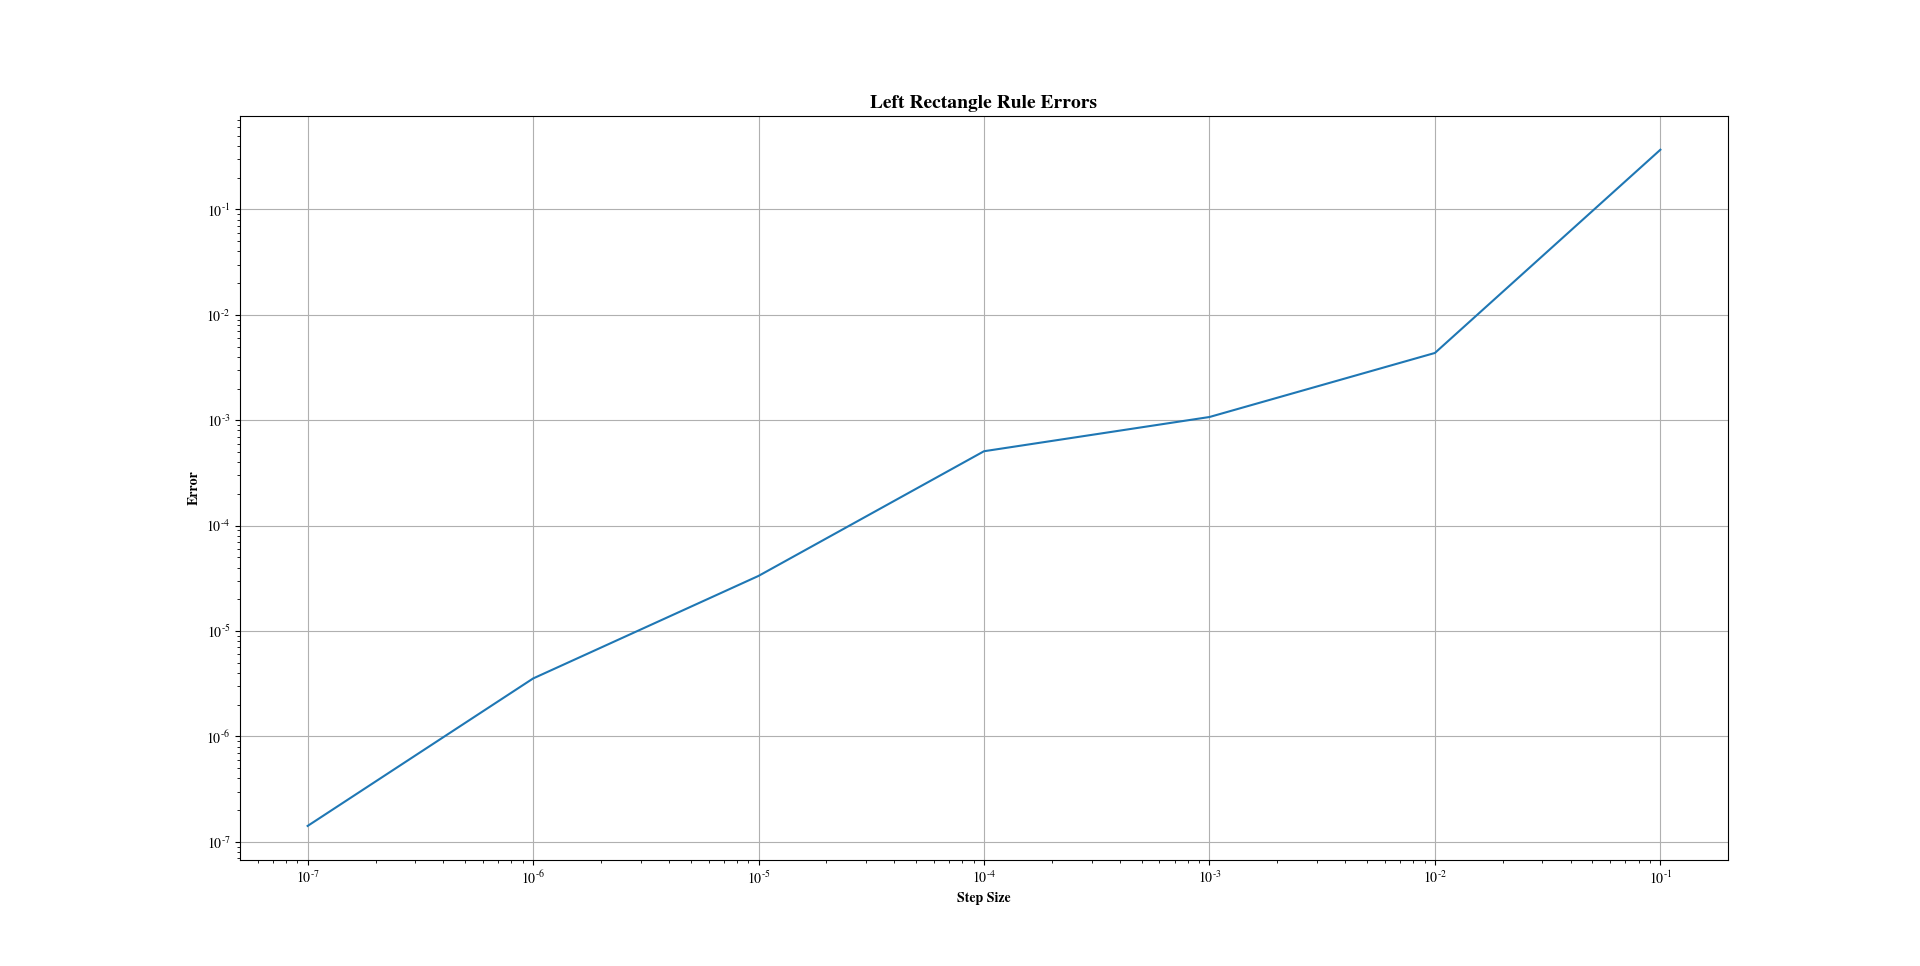
\includegraphics[width=1\textwidth,height=\textheight,keepaspectratio]{media/1/Figure_1.png}
		\end{subfigure}%

    	\begin{subfigure}[c]{.8\textwidth}
			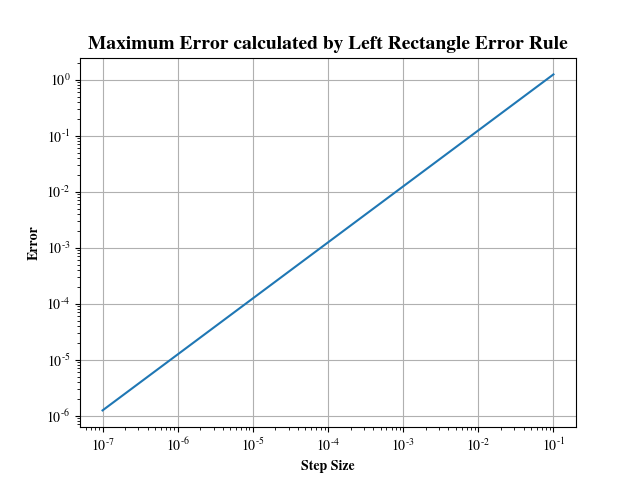
\includegraphics[width=1\textwidth,height=\textheight,keepaspectratio]{media/1/Figure_2.png}
		\end{subfigure}
	\end{adjustbox}
	\caption{Κανόνας Αριστερού Παραλληλογράμμου}
	
    \label{(Left_Rectangular_Rule)}
\end{figure}
\vspace*{\fill}

\newpage
\begin{figure}[H]
	\begin{adjustbox}{center}
		\begin{subfigure}[c]{.8\textwidth}    
			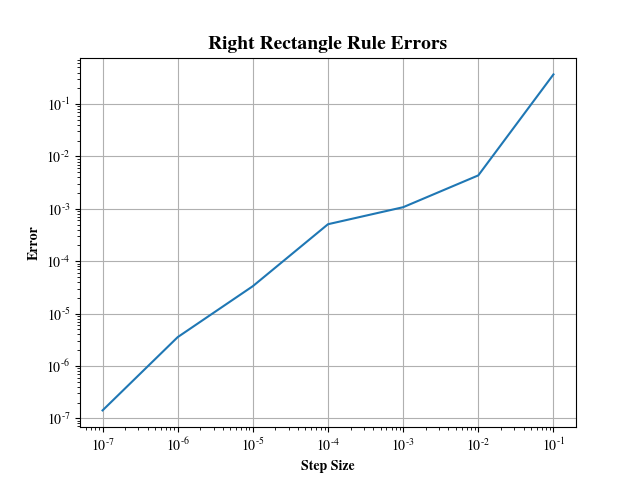
\includegraphics[width=1\textwidth,height=\textheight,keepaspectratio]{media/1/Figure_3.png}
		\end{subfigure}%

	    \begin{subfigure}[c]{.8\textwidth}    
			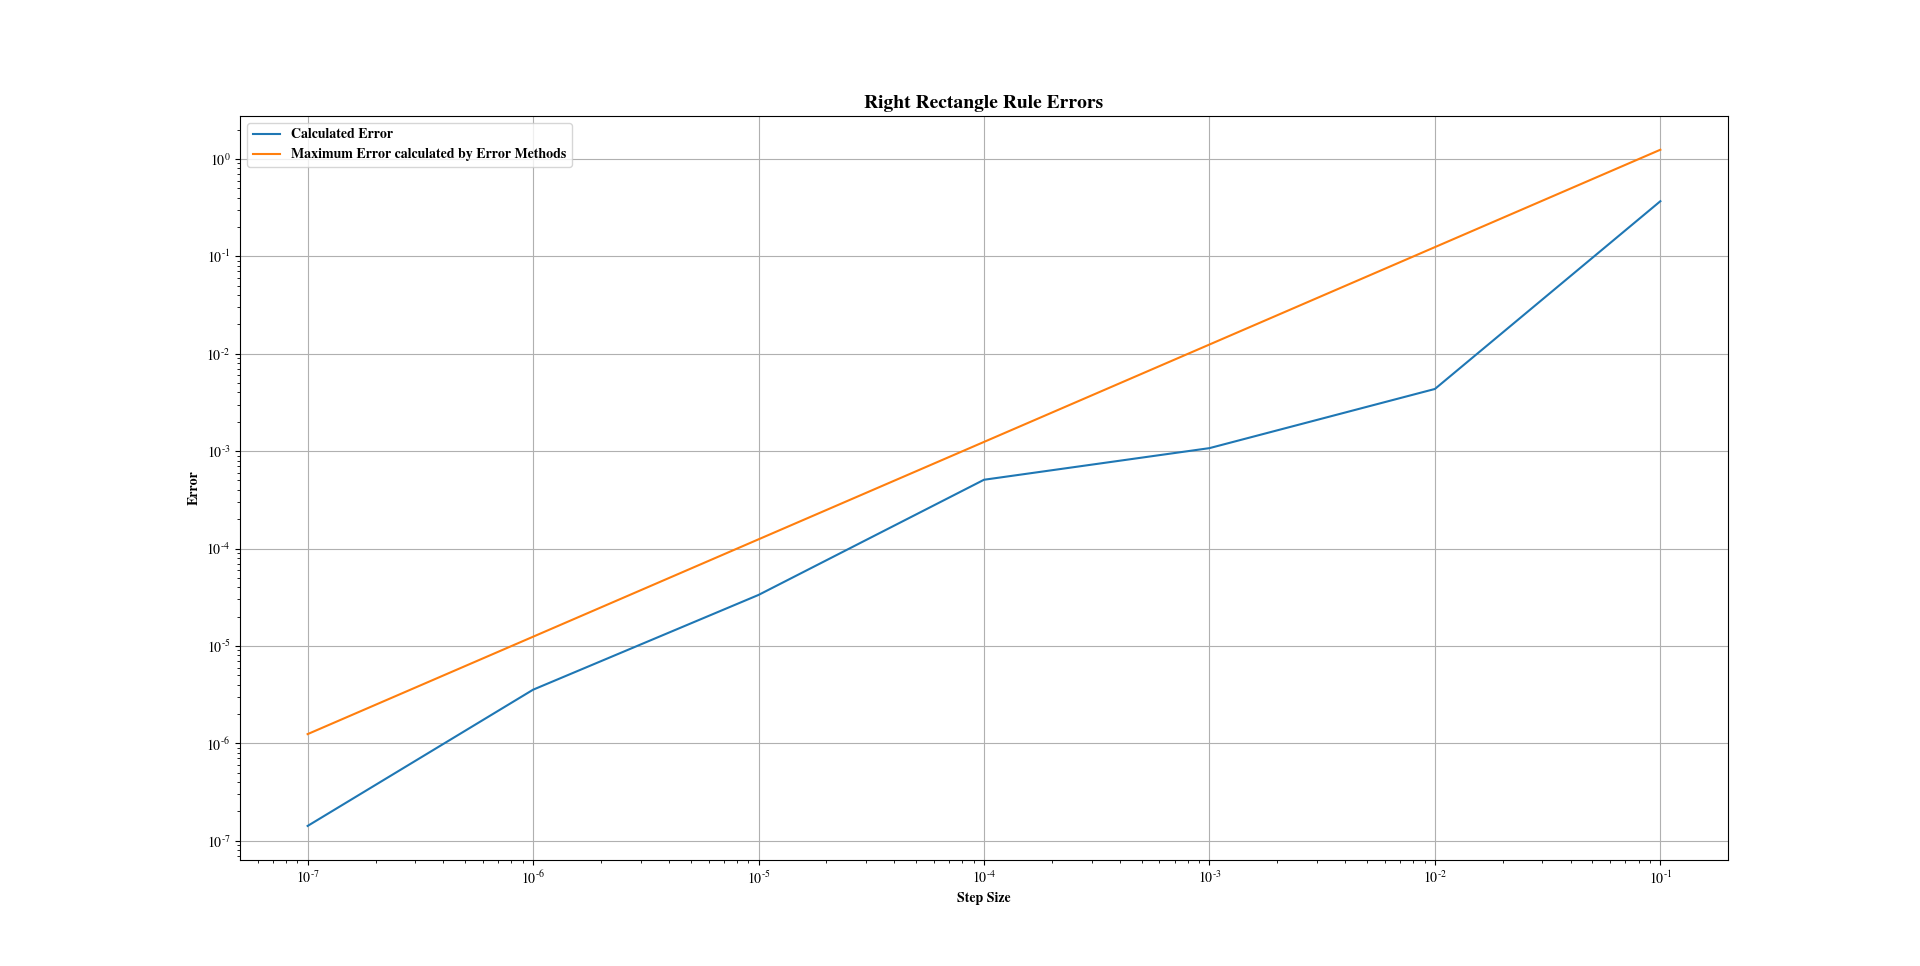
\includegraphics[width=1\textwidth,height=\textheight,keepaspectratio]{media/1/Figure_4.png}
		\end{subfigure}%
		
	\end{adjustbox}
\caption{Κανόνας Δεξιού Παραλληλογράμμου}
    \label{(Right_Rectangular_Rule)}
\end{figure}

\vspace*{\fill}
\begin{figure}[H]	
	\begin{adjustbox}{center}
		\begin{subfigure}[c]{.8\textwidth}    
			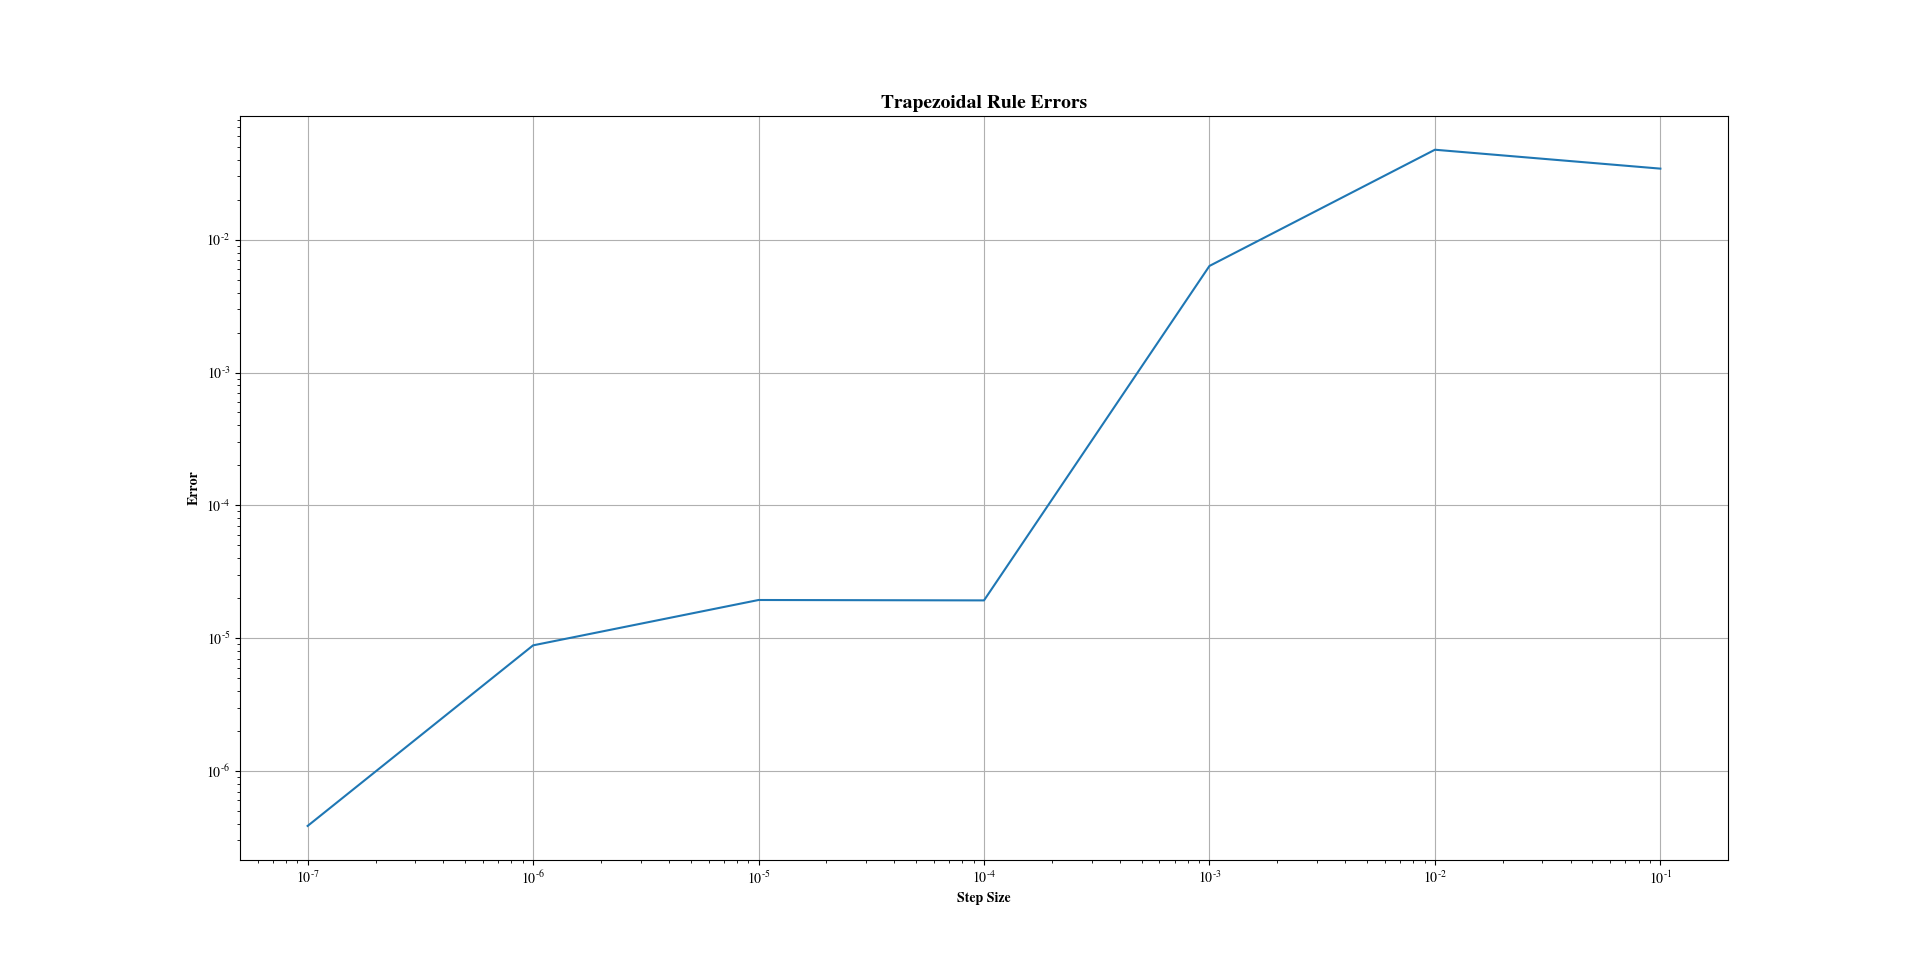
\includegraphics[width=1\textwidth,height=\textheight,keepaspectratio]{media/1/Figure_5.png}
		\end{subfigure}%

	\begin{subfigure}[c]{.8\textwidth}    
			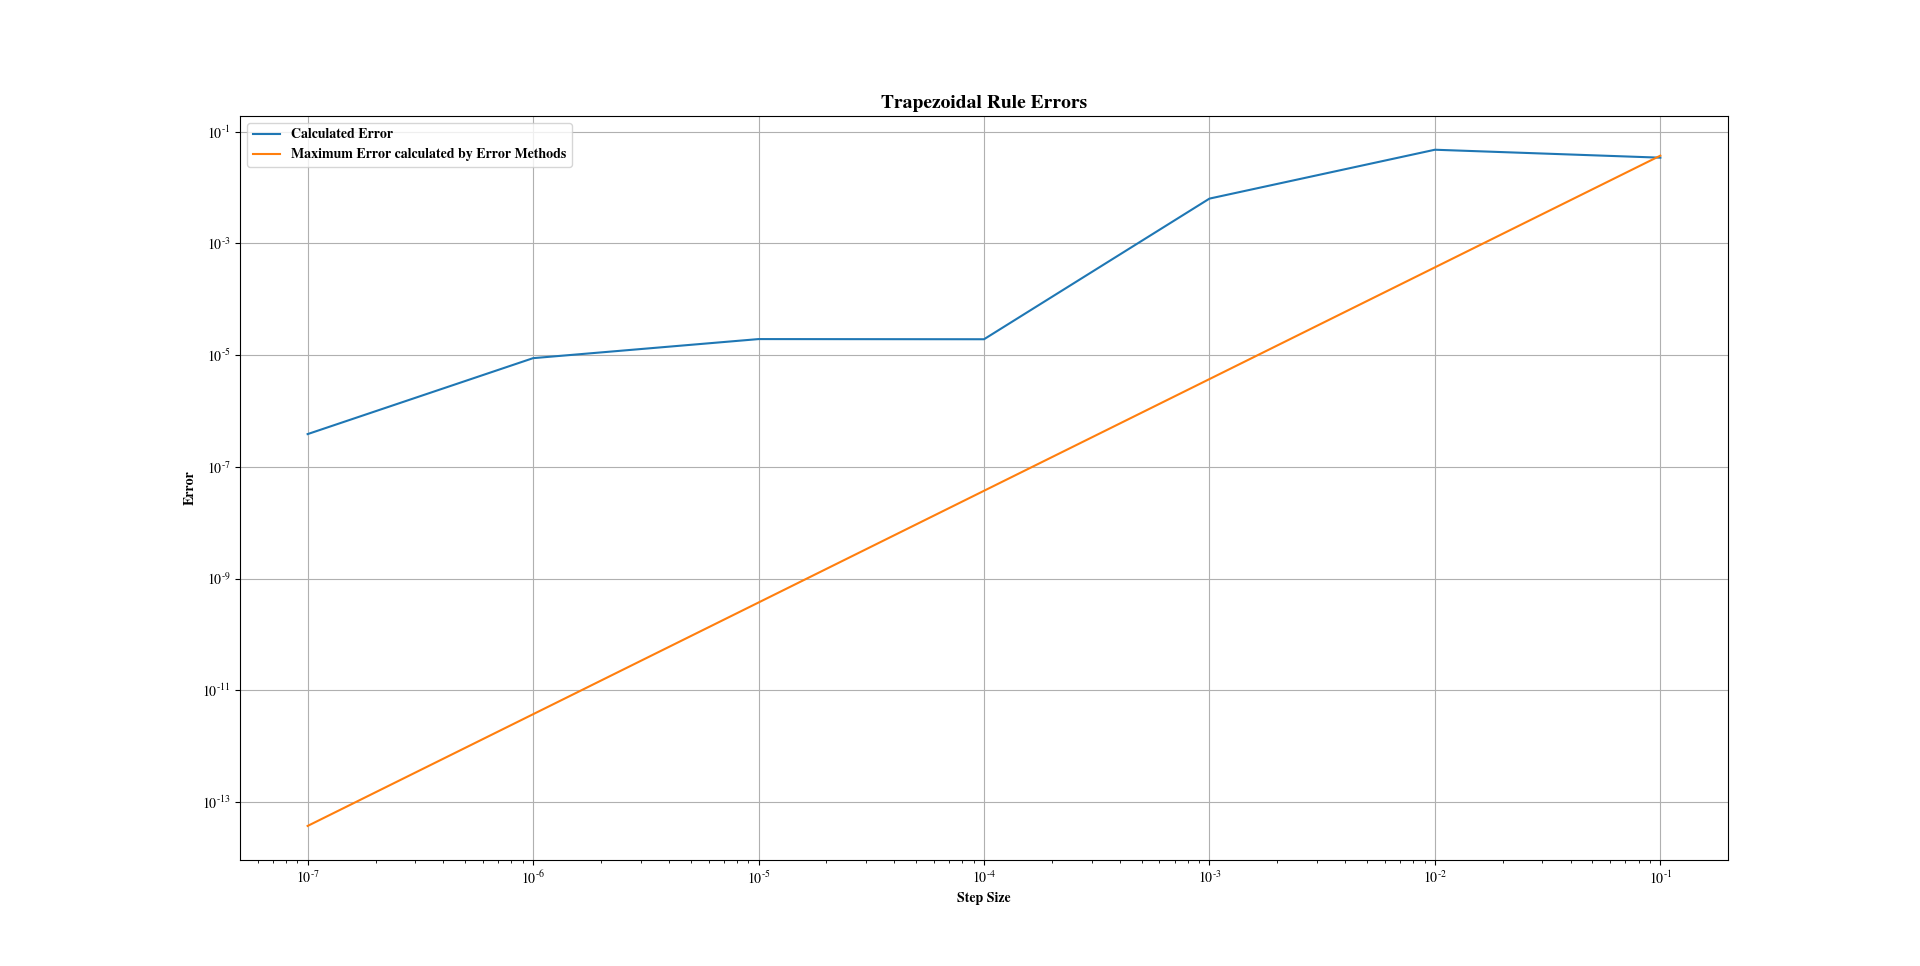
\includegraphics[width=1\textwidth,height=\textheight,keepaspectratio]{media/1/Figure_6.png}
		\end{subfigure}%
		
	\end{adjustbox}
\caption{Κανόνας Τραπεζίου}
\label{(Trapezoidal_Rule)}
\end{figure}

\vspace*{\fill}
\newpage
\begin{figure}[H]
    \centering	
	\begin{adjustbox}{center}
		\begin{subfigure}[c]{.8\textwidth}    
			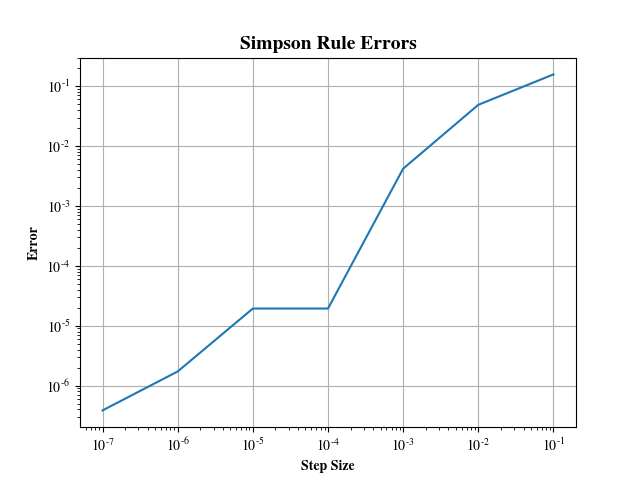
\includegraphics[width=1\textwidth,height=\textheight,keepaspectratio]{media/1/Figure_7.png}
		\end{subfigure}%

	\begin{subfigure}[c]{.8\textwidth}    
			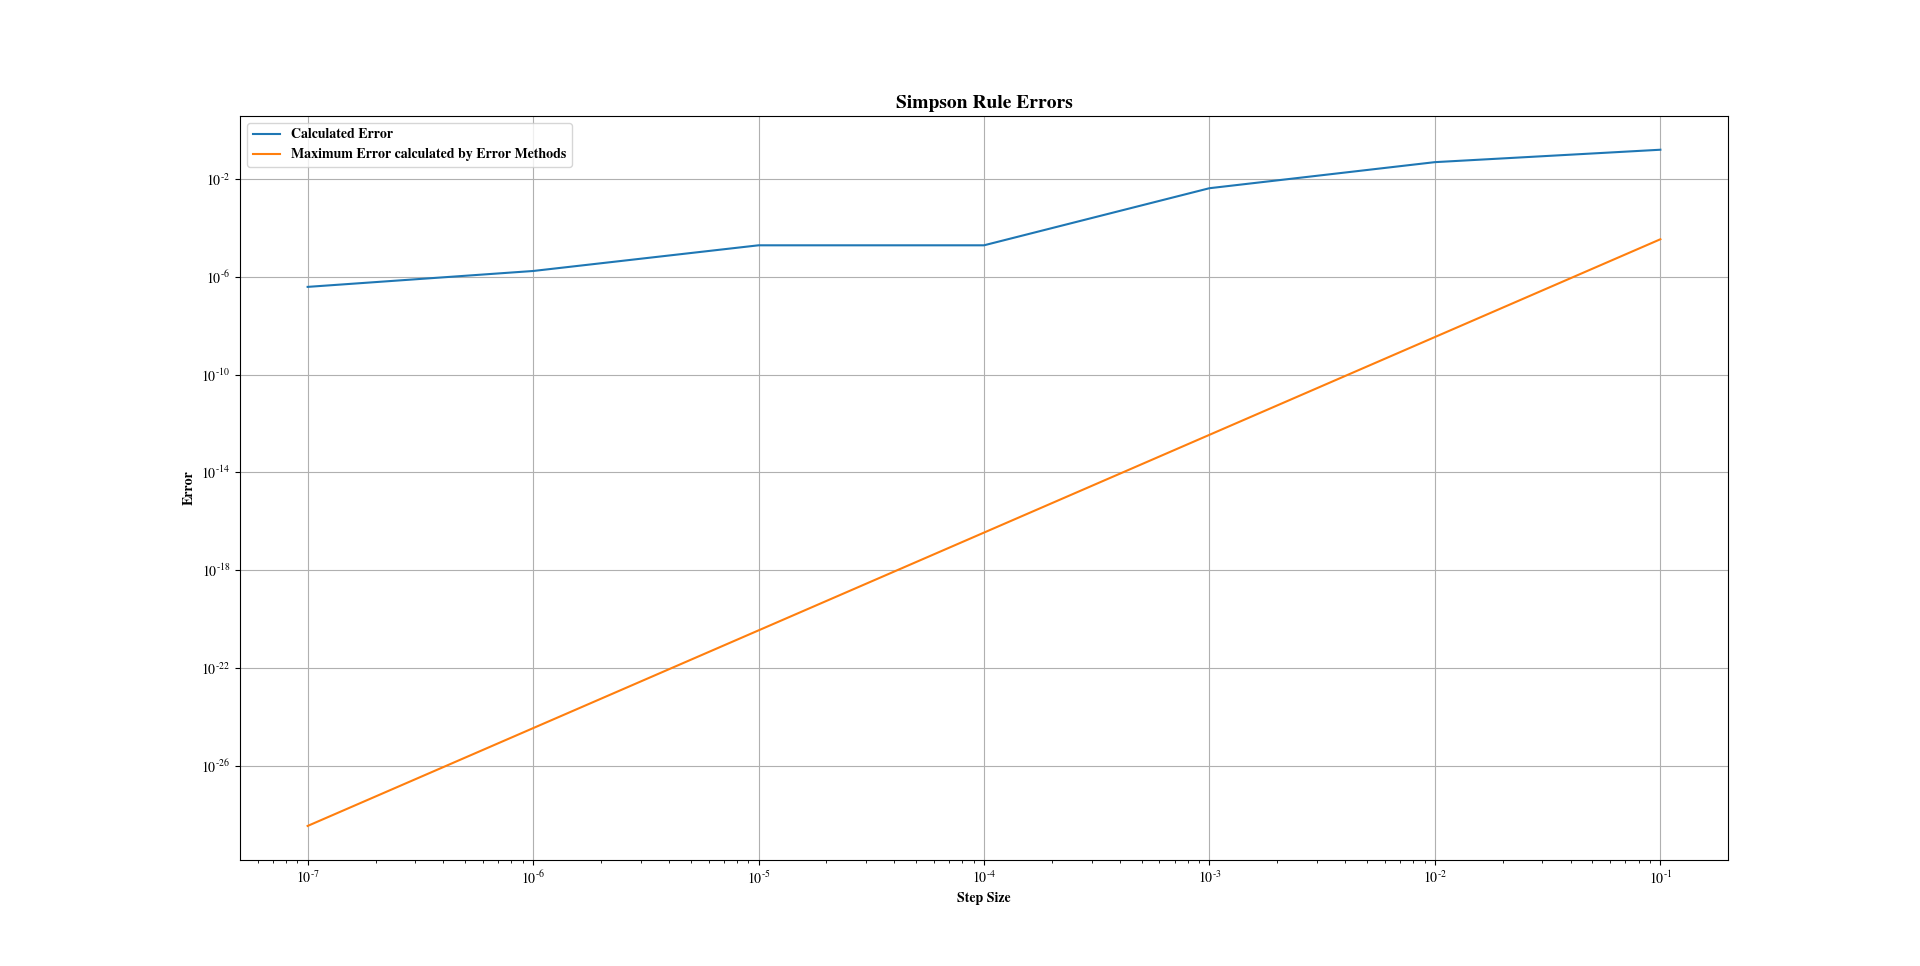
\includegraphics[width=1\textwidth,height=\textheight,keepaspectratio]{media/1/Figure_8.png}
		\end{subfigure}%
	\end{adjustbox}

\caption{Κανόνας \foreignlanguage{english}{Simpson}}
\label{(Simpson_Rule)}
\end{figure}

\vspace*{\fill}
\subsection{Ερώτημα γ}
Όπως αναμέναμε, το υπολογιζόμενο απόλυτο σφάλμα κάθε μεθόδου, όπως αυτό υπολογίζεται από το πραγματικό αποτέλεσμα της ολοκλήρωσης (το οποίο δόθηκε από την εκφώνηση) και την τιμή του ολοκληρώματος που προκύπτει με την χρήση των μεθόδων αριθμητικής ολοκλήρωσης είναι παντού μικρότερο από το μέγιστο σφάλμα, το οποίο δίνεται από τους κανόνες υπολογισμού σφάλματος των μεθόδων. 
\vspace*{\fill}
\newpage
\section{Εργασία 2}

\vspace*{\fill}

\subsection{Ερώτημα α}
Η υλοποίηση της μεθόδου του \foreignlanguage{english}{Euler} μπορεί να ευρεθεί στο αρχείο \foreignlanguage{english}{Differential\_Equation\_Method.py}.
\vspace*{\fill}
\subsection{Ερώτημα β}
Το πρόβλημα που αναφέρεται στην εκφώνηση μοντελοποιείται και επιλύεται στο αρχείο \foreignlanguage{english}{Differential\_Equations\_Problem\_Solving.py}. Όπως αναφέρουν οι οδηγίες της εκφώνησης χρησιμοποιούμε αρχικές συνθήκες $ x_0(0) = 20, x_1(0) = 1, t_{max} = 200 $ και μικρό βήμα διακριτοποίησης $ dt = 0.01 $.
\vspace*{\fill}
\subsection{Ερώτημα γ}
Στο \autoref{(dt=0.01)}, εμφανίζονται τα αποτελέσματα της επίλυσης της δοθείσας διαφορικής εξίσωσης. Στα αριστερά σχεδιάζεται η πληθυσμιακή εξέλιξη των δύο ειδών σε σχέχη με τον χρόνο. Στα δεξιά, απεικονίζεται η ανταλλαγή πληθυσμιακής κυριαρχίας.
\vspace*{\fill}
\begin{figure}[H]
    \centering
	\begin{adjustbox}{center}

		\begin{subfigure}[c]{0.8\textwidth}    
			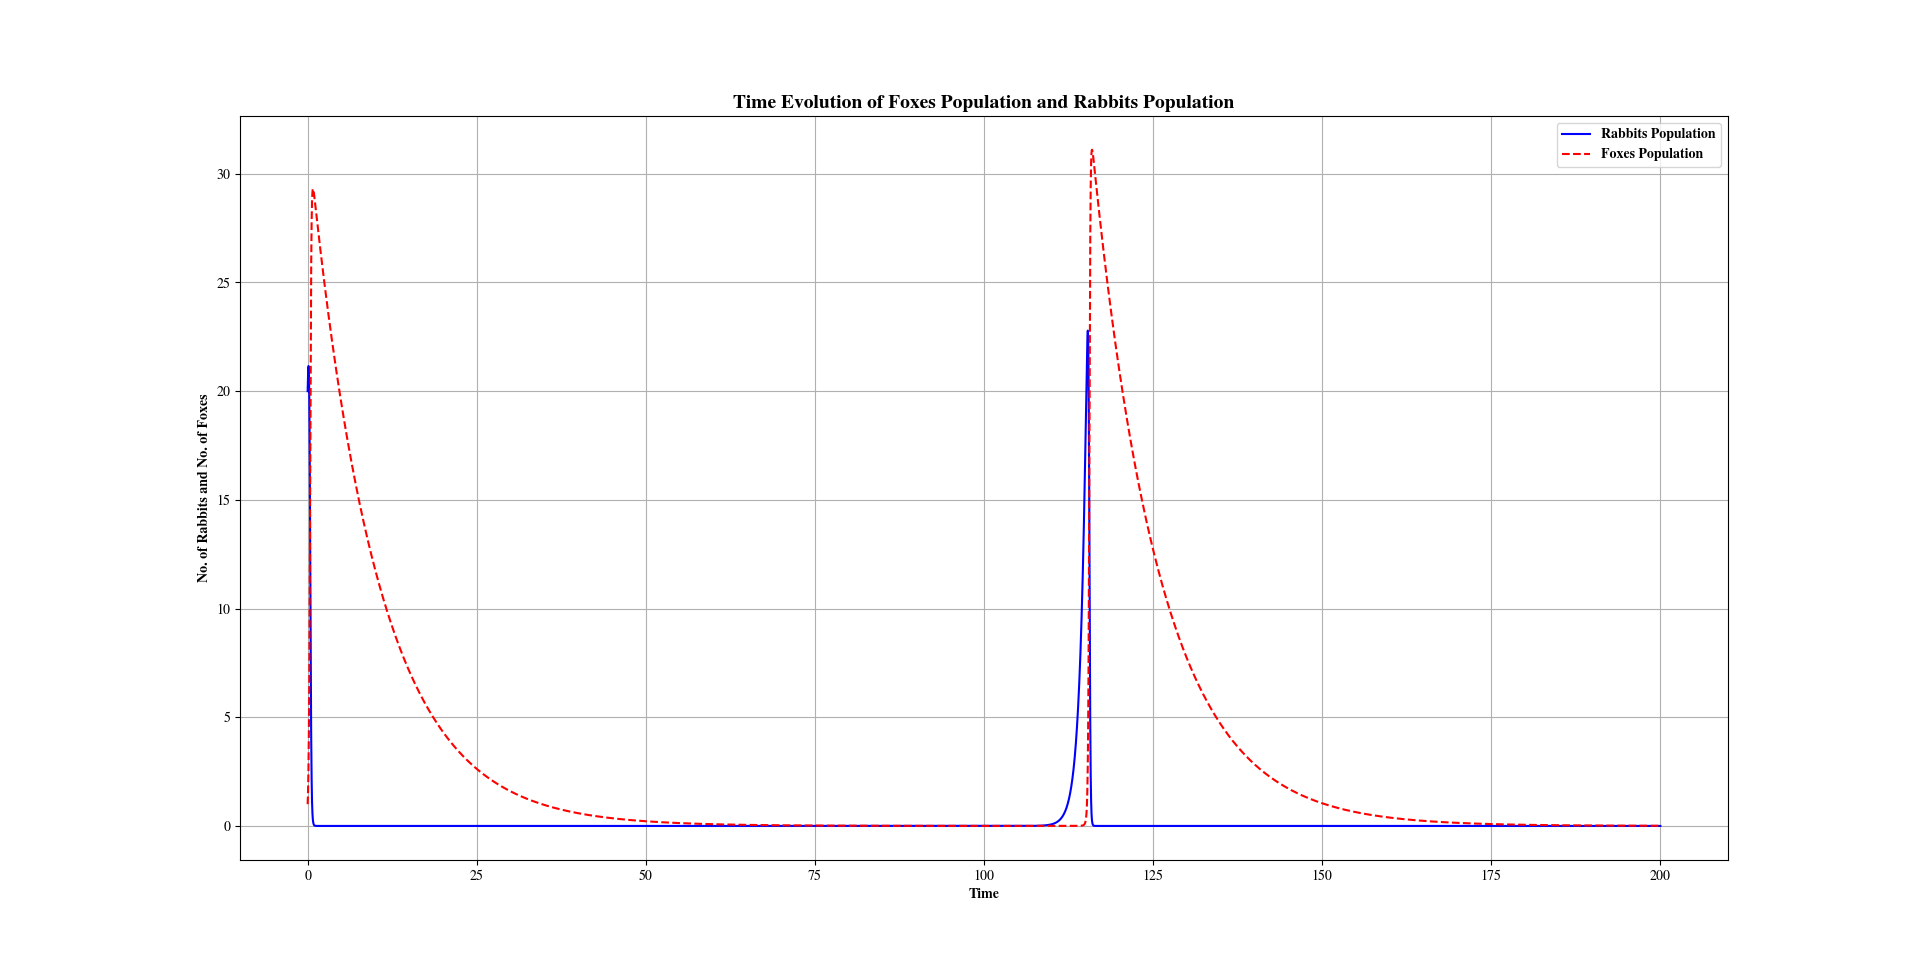
\includegraphics[width=1\textwidth,height=\textheight,keepaspectratio]{media/2/dt=0.01/Figure_1.png}
		\end{subfigure}
		
    	\begin{subfigure}[c]{.8\textwidth}
			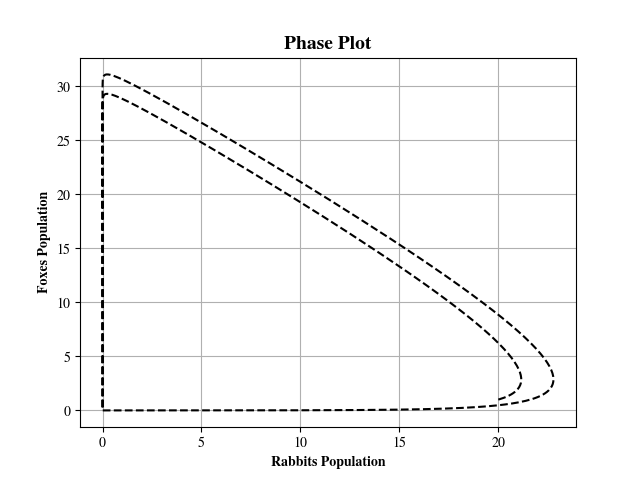
\includegraphics[width=1\textwidth,height=\textheight,keepaspectratio]{media/2/dt=0.01/Figure_2.png}
		\end{subfigure}
	\end{adjustbox}
\caption{Βήμα Διακριτοποίησης 0.01}
\label{(dt=0.01)}
\end{figure}
\vspace*{\fill}
\newpage
\noindent
Όπως είναι εμφανές στο \autoref{(dt=0.01)}, η πληθυσμιακή εξέλιξη των λαγών εξαρτάται άμεσα από αυτήν των αλεπούδων και αντίστροφα. Πιο συγκεκριμένα, αύξηση των λαγών συνεπάγεται την ραγδαία εκθετική αύξηση των αλεπούδων. Από την άλλη, μείωση των λαγών οδηγεί σε εκθετική μείωση (με μικρότερη κλίση συγκριτικά με αυτή της αύξησης) των αλεπούδων, ενώ αύξηση των αλεπούδων οδηγεί στην μείωση των λαγών. Το μοτίβο επαναλαμβάνεται περιοδικά. Επιπροσθέτως, ο μέγιστος αριθμός ατόμων κάθε είδους δείχνει να αυξάνεται με την πάροδο του χρόνου, όπως φαίνεται στο \autoref{(max)}, στο οποίο το $ t\_{max} $ είναι ίσο με 400.

\begin{figure}[H]
    \centering
	\begin{adjustbox}{center}
	
		\begin{subfigure}[c]{1.2\textwidth}    
			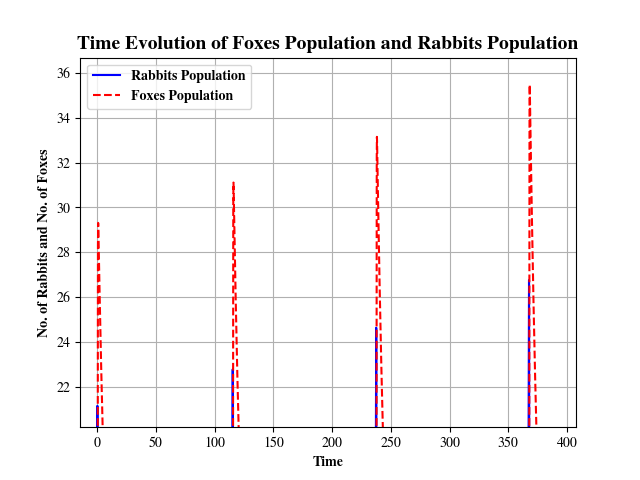
\includegraphics[width=1.2\textwidth,height=\textheight,keepaspectratio]{media/2/Figure_1.png}
		\end{subfigure}%

	\end{adjustbox}
\caption{Μέγιστα πληθυσμών συναρτήσει του χρόνου}
\label{(max)}
\end{figure}
\vspace*{\fill}
\subsection{Ερώτημα δ}

\noindent
\\
Μειώνουμε το βήμα διακριτοποίησης στο $\frac{1}{10}$ της προηγούμενης τιμής ($ dt = 0.001 $) και επαναλαμβάνουμε την επίλυση της διαφορικής εξίσωσης. Τα αποτελέσματα για το νέο $ dt $ φαίνονται στα παρακάτω γραφήματα.
\newline
\newline
\begin{figure}[H]
    \centering
	\begin{adjustbox}{center}
		\begin{subfigure}[c]{.8\textwidth}    
			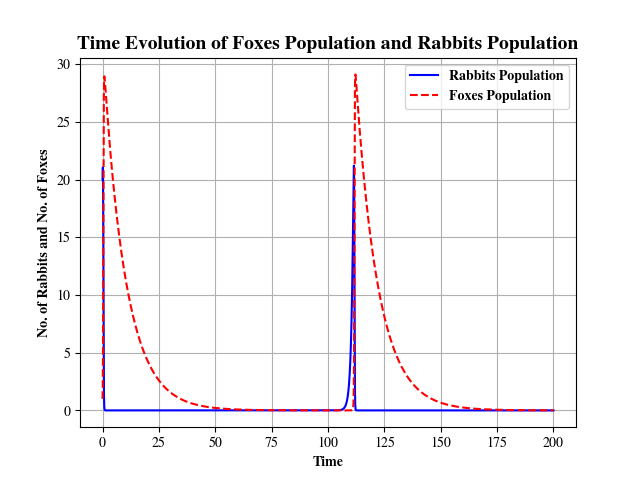
\includegraphics[width=1\textwidth,height=\textheight,keepaspectratio]{media/2/dt=0.001/Figure_1.png}
		\end{subfigure}%

	    \begin{subfigure}[c]{.8\textwidth}    
			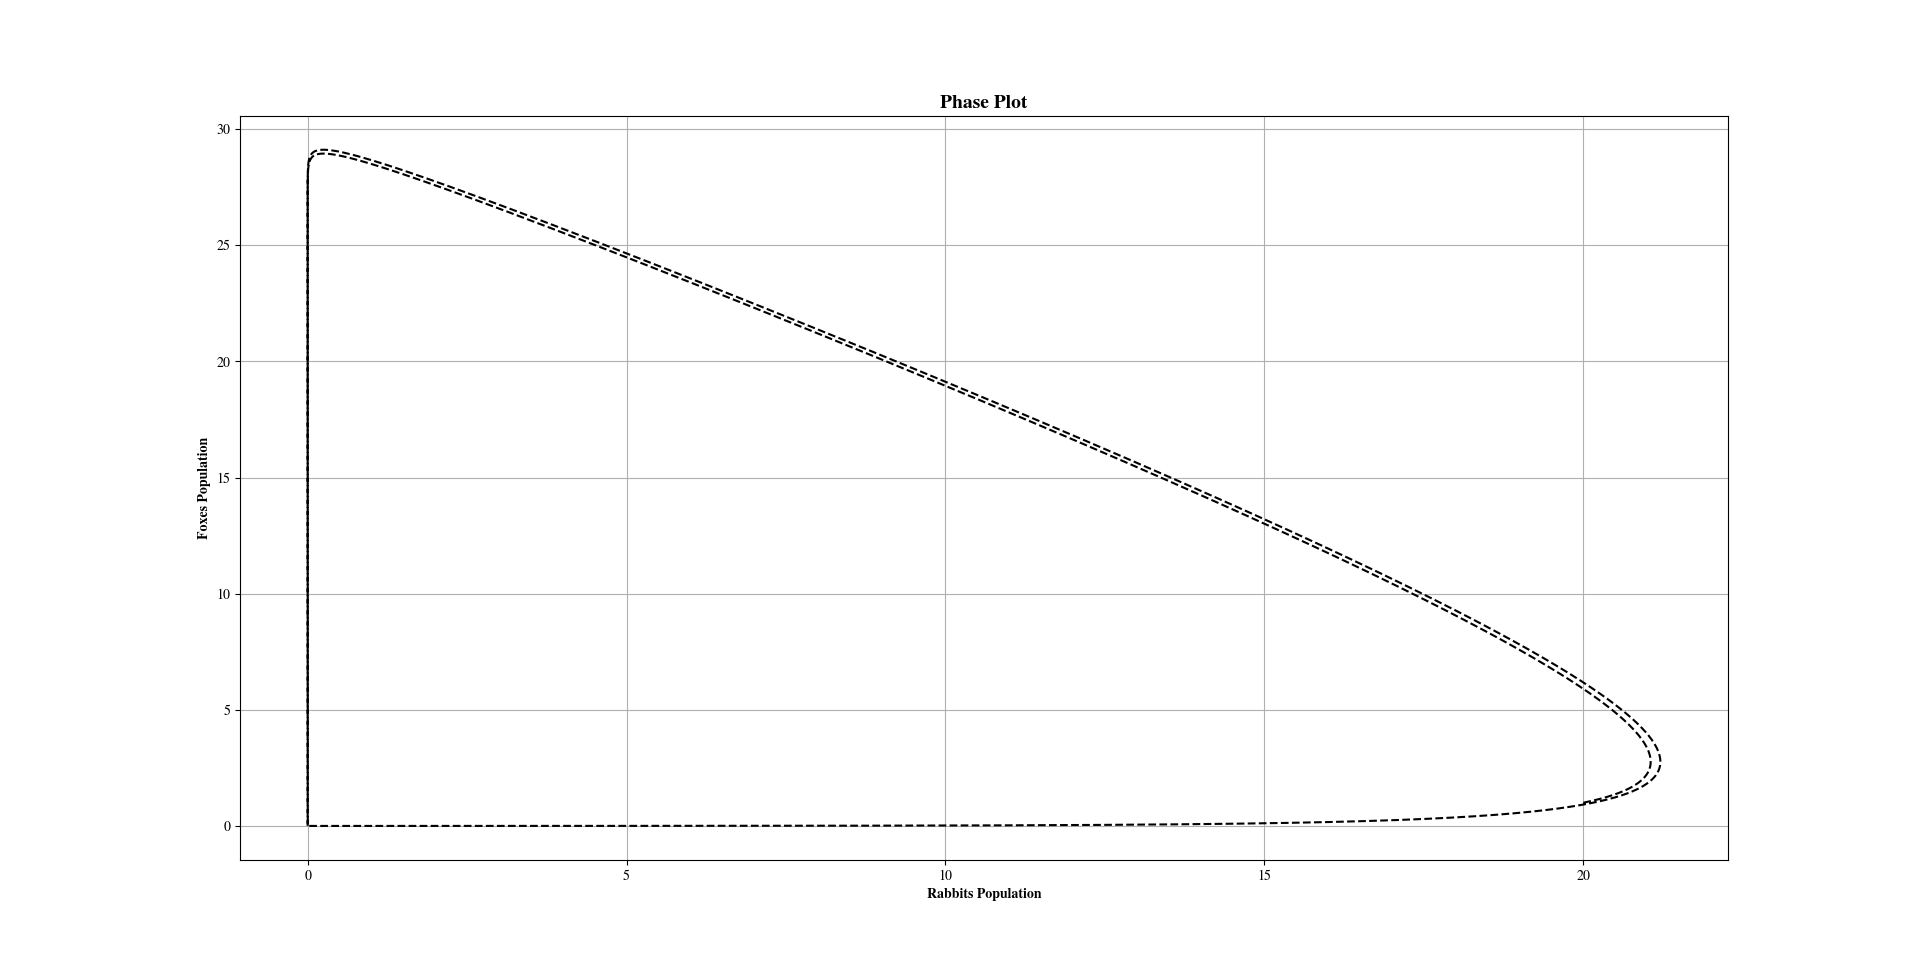
\includegraphics[width=1\textwidth,height=\textheight,keepaspectratio]{media/2/dt=0.001/Figure_2.png}
		\end{subfigure}%
	\end{adjustbox}
\caption{Βήμα Διακριτοποίησης 0.001}
\label{(dt=0.001)}
\end{figure}

\noindent
\\
\\
\\
Όσον αφορά το πρώτο γράφημα παρατηρούμε ότι η πληθησμιακή αύξηση που παρατηρείται για $ dt = 0.01 $ δεν είναι πλέον τόσο έντονη. Παράλληλα,  υπάρχει μια μικρή χρονική μετατόπιση όσον αφορά την περιοδικότητα του φαινομένου.

\noindent
\newline
Το γράφημα στα αριστερά παρουσιάζει και αυτό διαφορές συγκριτικά με το \foreignlanguage{english}{Phase Plot} (\autoref{(dt=0.01)}) του προηγούμενου ερωτήματος. Φαίνεται ότι η επανάληψη του φαινομένου δεν συνεπάγεται πλεόν την ραγδαία αύξηση πληθυσμών. 

\end{document}